\section{Bridge}

\begin{figure}
\center
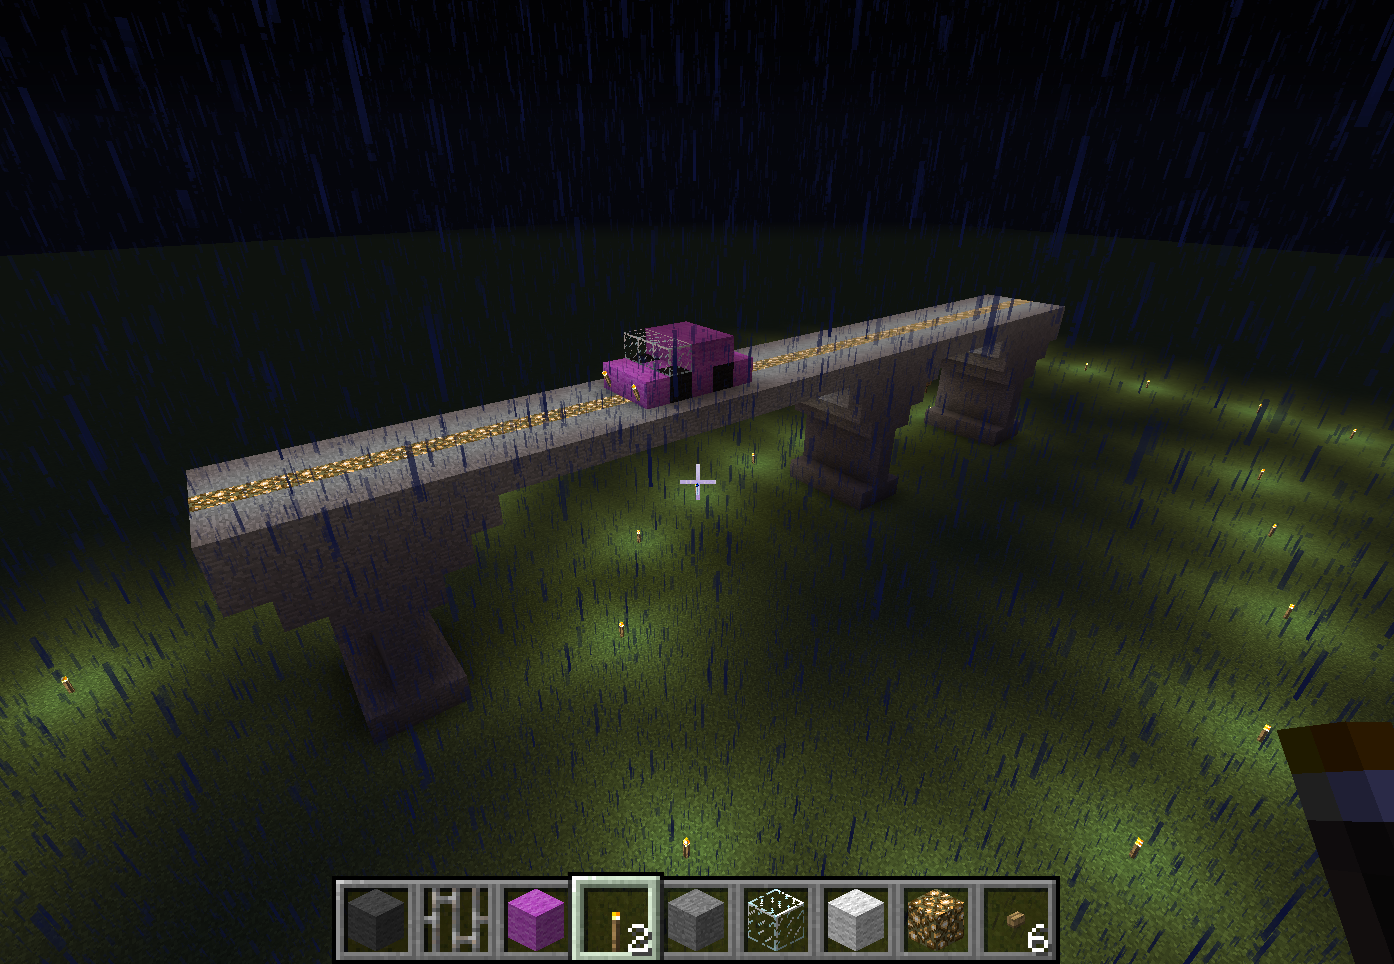
\includegraphics[trim=0cm 5cm 7cm 7cm, clip=true, width=0.7\textwidth]{pic_bridge}
\caption{A picture of the bridge we built in minecraft.}
\label{fig:picBridge}
\end{figure}


For this section we ventured ahead and built ourselves a bridge in minecraft as shown in Figure \ref{fig:picBridge}. Importing the bridge into matlab was, apart from some tedious work, quite straight forward.


\subsection{Short overview of algorithm}
Since we wanted to have some kind of time-dependency on our chosen problem, we incorporated a car driving over the bridge. This required us to manually link together the meshes for the bridge and car, and is done in the \textit{mergeBridgeCar.m} matlab function. The supplied \textit{hex2tetr.m} function is used to split our minecraft cubes into fitting tetrahedrons. We find the boundary points at $z = 0$, and pass the whole thing into \textit{FEM.m} which solves the linear elasticity problem using the finite element method further specified in Section \ref{sec:FEM}. The function \textit{stressRecovery.m} recovers the nodal Von Mises stresses by averaging the element neighbor stresses for each node. The stress is found by \eqref{stress-displacement}.


\subsection{Materials chosen}
\begin{table}
\center
\caption{Material constants for oak wood used in the bridge.} 
\begin{tabular}{cc}
Material constant & Value \\ 
\hline \noalign{\smallskip}
Young's modulus & 11 GPa \\ 
Density & 650 kg/m$^3$ \\ 
Compressive yield strength & 46 MPa \\ 
Poissons ratio & 0.3 \\ 
\label{tab:oak}
\end{tabular}
\end{table}


For this problem we chose the material of the bridge to be oak wood. We defined the dimension of one minecraft block to be a cubic meter. The material constants we needed for wood were the averaged values we found at \cite{oak} and the value for the Poisson's ratio was conveniently set to 0.3. All the material constants are presented in table \ref{tab:oak}. We really wanted to see what happens when a heavy car drives over the bridge, so we defined the car to be extremely heavy. The result of this is visualized in Figure \ref{fig:bridget8t23}.

\subsection{Results}
The resulting Von Mises stress plot at two different times are plotted in figure \ref{fig:bridget8t23}. A video of the car as it moves over the bridge is also produced, but is obviously not included in this text report.

\begin{figure}[ht]
        \centering
        \begin{subfigure}[b]{0.45 \textwidth}
                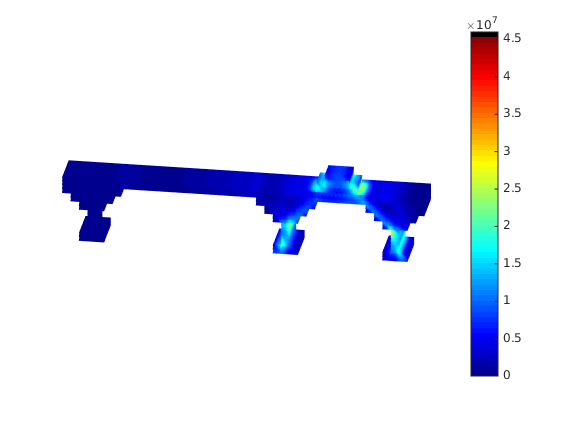
\includegraphics[width=\textwidth]{time080}
                \caption{The car after 8 seconds have passed.}
        \end{subfigure}
        ~
        \begin{subfigure}[b]{0.45 \textwidth}
                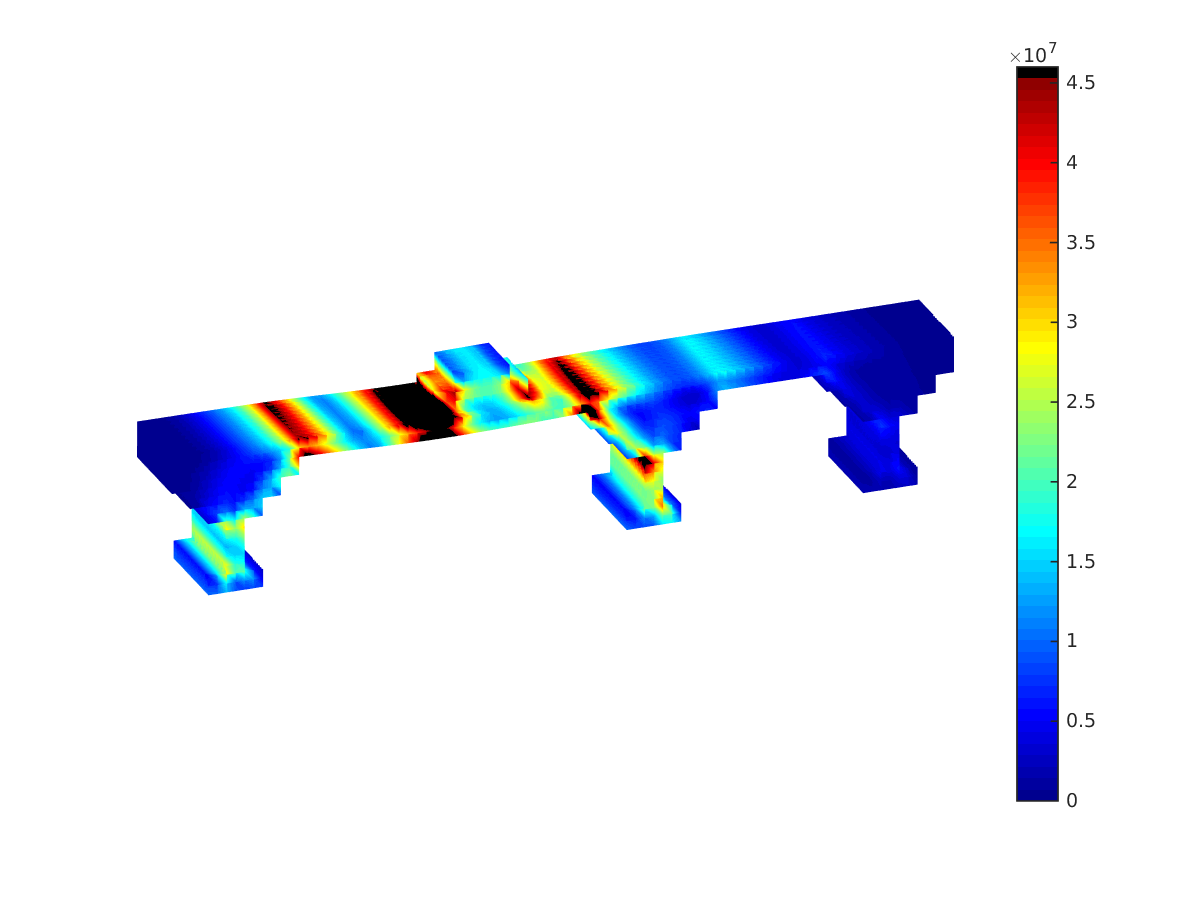
\includegraphics[width=\textwidth]{time230}
                \caption{The car after 28 seconds have passed.}
        \end{subfigure}
        \caption{The (really) heavy car driving over the bridge at 1 m/s. The Von Mises stress is plotted as the varying color. If the Von Mises stress is higher than the material yield, it is painted black (and the bridge will be permanently deformed). We see that at time = 28 the bridge has been severely damaged. }
        \label{fig:bridget8t23}
\end{figure}

